
\begin{lead}
 前章では,正弦波信号をシステムに加えた場合の応答として周波数特性を説明した.しかし,実際のシステムへの入力信号が正弦波信号であることは少ない.このような場合,正弦波以外の信号が正弦波とどのような関係にあるかを調べる必要がある.このような操作を周波数解析という.周波数解析はアナログ信号とそのサンプル値との関係に関する重要な定理であるサンプリング定理を理解するためにも必要なことである.


\end{lead}

%\vfill

%\begin{koumoku}
%周波数解析\\
%正弦波信号\\
%アナログ信号\\
%サンプル値\\
%サンプリング定理\\
%\end{koumoku}

%\clearpage


\chapter[信号の周波数解析とサンプリング定理]{信号の周波数解析と\\サンプリング定理}
\label{chapter:6}

\section{\index{しゅうはすうかいせき@周波数解析}周波数解析}

解析しようとする信号が正弦波であれば,取り扱いは比較的容易であるとされている.ところが,ディジタル信号を含め一般的に扱われる信号は,周期的であったとしても正弦波のような形状の信号ではないことがほとんどであり,これを非正弦波信号と呼んでいる.ここではその取り扱いについて説明する.

\subsection{非正弦波信号}

図\ref{fig:zu_4-1}(a)に示すアナログ信号$x_{T_0}(t)$を例に説明する.この信号は正弦波信号の負の値を切り捨てたものであり,もはや正弦波信号ではない.このような正弦波以外の信号を\index{ひせいげんはしんごう@非正弦波信号}非正弦波信号という.非正弦波信号は,周波数,大きさ,位相の異なる複数の\index{せいげんはしんごう@正弦波信号}正弦波信号の合成として表現される.

たとえば,図\ref{fig:zu_4-1}(a)の信号は,次式のように無限個の正弦波信号を用いて表現される.

\begin{eqnarray}
x_{T_0}(t)&=&\frac{1}{\pi} + \frac{1}{2} \cos \Omega_0 t %\nonumber \\
 + \frac{2}{\pi} \left ( \frac{1}{1 \times 3} \cos (2\Omega_0 t) - \frac{1}{3 \times 5} \cos (4\Omega_0 t) \right )
\label{eqn:04-1}
\end{eqnarray}

\begin{figure}[H]
\begin{center}
\begin{minipage}{.32\textwidth}
\begin{center}
%\includegraphics[width=8cm]{fig/fig-4-1.eps}
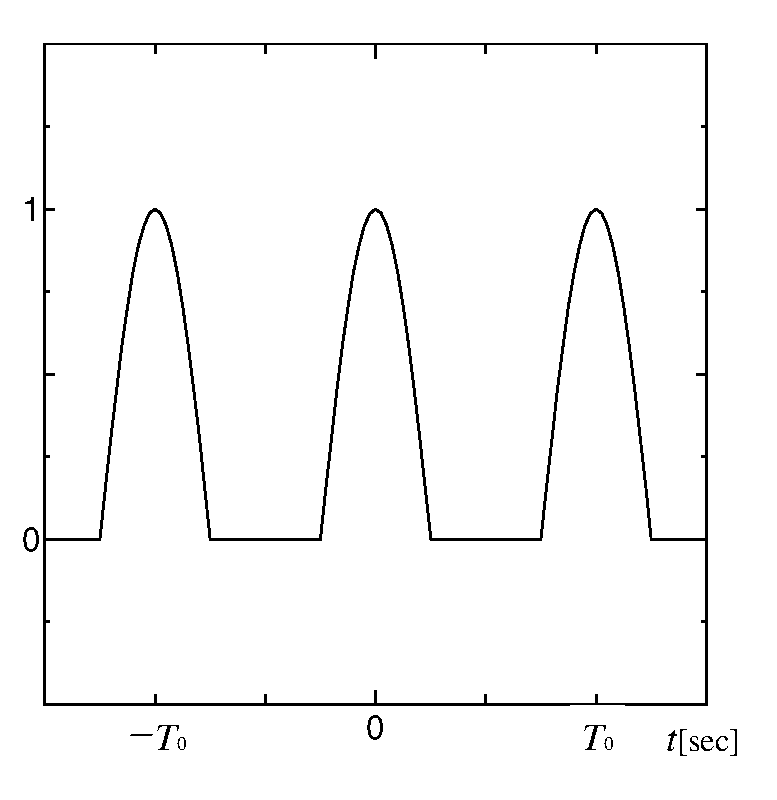
\includegraphics[width=.98\textwidth]{fig/fig-4-1-a.eps}

(a)
\end{center}
\end{minipage}
\begin{minipage}{.32\textwidth}
\begin{center}
%\includegraphics[width=8cm]{fig/fig-4-1.eps}
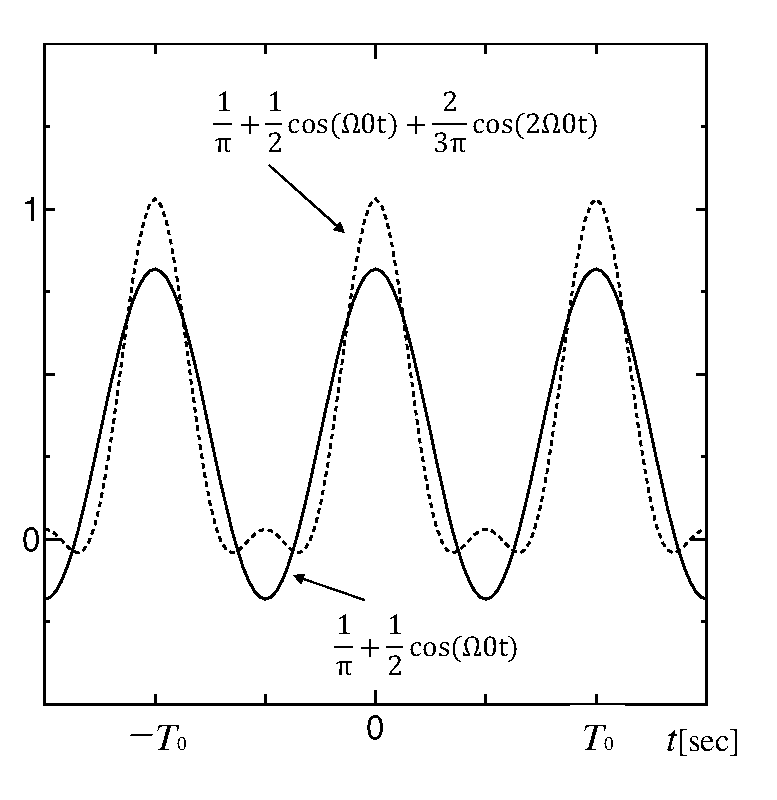
\includegraphics[width=.98\textwidth]{fig/fig-4-1-b.eps}

(b)
\end{center}
\end{minipage}
\end{center}\vskip.32\baselineskip
\caption{非正弦波信号の例}
\label{fig:zu_4-1}
\end{figure}

\noindent ただし,$\Omega_0 = 2\pi / T_0$である.図\ref{fig:zu_4-1}(b)は,式(\ref{eqn:04-1})の有限個数の項の正弦波信号を加算して合成された信号である.合成される正弦波信号の項数が増えると,図\ref{fig:zu_4-1}(a)のような波形に外形が近づいてきていることがわかる.

このように,たとえば図\ref{fig:zu_4-1}(a)の信号を式(\ref{eqn:04-1})のように展開するように非正弦波信号を正弦波信号に分解し,信号の性質を調べる操作を周波数解析という.この正弦波分解に基づく周波数分析を,特にフーリエ解析(Fourier analysis)という.

\subsection{フーリエ解析の種類}

フーリエ解析にはいくつかの種類がある.解析される信号のちがいにより,それらを使い分けなければならない.ここでは,まず\index{ふーりえかいせき@フーリエ解析}フーリエ解析の種類と対象とする信号との関係をまとめる.

信号は図\ref{fig:zu_4-2}に示すように,離散時間信号か連続時間信号か,またそれぞれについて周期的か非周期的かにより大別され,信号の種類により,表\ref{table:table-4-1}に示すような5種類の\index{ふーりえかいせきほう@フーリエ解析法}フーリエ解析法が知られている.連続時間信号に対しては,\index{ふーりえへんかん@フーリエ変換}フーリエ変換(Fourier Transform: FT)と\index{ふーりえきゅうすう@フーリエ級数}フーリエ級数(Fourier Series: FS)表現がある.一方,離散時間信号に対しては,\index{りさんじかんふーりえへんかん@離散時間フーリエ変換}離散時間フーリエ変換(Discreate-Time Fourier Transform: DTFT)と\index{りさんじかんふーりえきゅうすう@離散時間フーリエ級数}離散時間フーリエ級数(Discreate-Time Fourier Series: DTFS)表現がある.

\begin{figure}[H]
\begin{center}
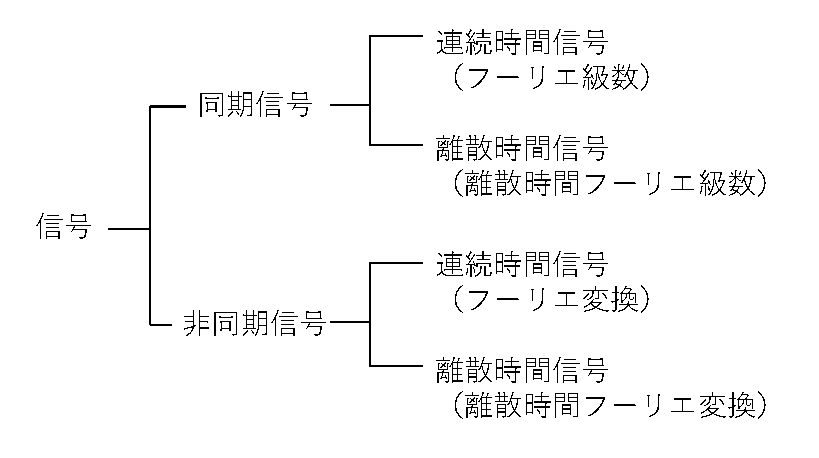
\includegraphics[width=.7\textwidth]{fig/fig-4-2.eps}
\end{center}
\caption{信号の分類と対応するフーリエ解析}
\label{fig:zu_4-2}
\end{figure}


\begin{table}
\caption{フーリエ解析の種類}
\begin{center}
\begin{tabular}{|c|c|c|}
\hline
 & 離散時間信号 & 連続時間信号 \\
\hline
\begin{minipage}{3mm}\centering
周 \\ 期 \\ 信 \\ 号
\end{minipage}
 &
\begin{minipage}{5cm}\vskip 2mm
\begin{center}
$\displaystyle x_N(n)=\frac{1}{N}\sum_{k=0}^{N-1}X_N(k)W_N^{-nk}$ \\
($-\infty < n < \infty$) \\
$\displaystyle X_N(k)=\sum_{n=0}^{N-1}x_N(n)W_N^{-nk}$ \\
($-\infty < k < \infty$) \\
離散フーリエ変換\vspace*{2mm}
\end{center}
\end{minipage}
 &
\begin{minipage}{5cm}
\begin{center}
$\displaystyle x_{T_0}(t)=\sum_{k=-\infty}^{\infty}C_k e^{jk \Omega_0 t}$ \\
$\displaystyle C_k=\frac{1}{T_0}\int_{0}^{T_0}x_{T_0}(t) e^{-jk \Omega_0 t} dt$ \\
フーリエ級数
\end{center}
\end{minipage}
\\ \hline
\begin{minipage}{3mm}\centering
 \\ \\ 非 \\ 周 \\ 期 \\ % 信 \\ 号 \\}
\end{minipage}
 &
\begin{minipage}{5cm}\vskip 2mm
\begin{center}
$\displaystyle x(n)=\frac{1}{2\pi}\int_{0}^{2\pi}X(e^{j\omega})e^{j\omega n} d\omega$ \\
$\displaystyle X(e^{j\omega})=\sum_{n=-\infty}^{\infty}x(n)e^{-j\omega n}$ \\
離散時間フーリエ変換\vspace*{2mm}
\end{center}
\end{minipage}
 &
\begin{minipage}{5cm}
\begin{center}
$\displaystyle x(t)=\frac{1}{2\pi}\int_{-\infty}^{\infty}X(e^{j\omega})e^{j\omega n} d\omega$ \\
$\displaystyle X(\Omega)=\int_{-\infty}^{\infty}x(t)e^{-j\Omega t} dt$ \\
フーリエ変換
\end{center}
\end{minipage}
\\ \cline{2-3}
\begin{minipage}[b]{3mm}\centering
%非同期
\raisebox{2.8\baselineskip}[0mm][0mm]{信}\\
\raisebox{2.8\baselineskip}[0mm][0mm]{号}%
%\ \vspace*{-3\baselineskip}\par 信 \\ 号 \\ \\ \\
\end{minipage}
 &
\begin{minipage}{5cm}\vskip 2mm
\begin{center}
$\displaystyle x(n)=\frac{1}{N}\sum_{k=0}^{N-1}X(k)W_N^{-nk}$ \\
($n=0,1, \ldots , N-1$) \\
$\displaystyle X(k)=\sum_{n=0}^{N-1}x(n)W_N^{nk}$ \\
($k=0,1, \ldots , N-1$) \\
離散フーリエ変換\vspace*{2mm}
\end{center}
\end{minipage}
 &
%\begin{center}
\begin{minipage}{3cm}
ただし \\
$W_N = e^{-j2\pi/N}$ \\
$\Omega_0 = 2\pi/T_0$
\end{minipage}
%\end{center}
\\ \hline
\end{tabular}
\end{center}
\label{table:table-4-1}
\end{table}

\section{フーリエ級数}

ここでは,ある周期的な信号$f(t)=f(t+nT)$($n$は任意の整数)を考える.このとき,$f(t)$を基本角周波数$\omega_0$の整数倍による三角関数からなる級数で表すと,次式のように表される.
\begin{equation}
f(t)=\frac{a_o}{2}+\sum_{n=1}^{\infty}(a_n \cos n\omega_0 t + b_n \sin n\omega_0 t)
\label{eqn:fourier-kyusu_6}
\end{equation}
この式(\ref{eqn:fourier-kyusu_6})を実フーリエ級数と呼んでいる.ここで基本角周波数$\omega_0$(単位は[rad/s])は,
\begin{equation}
\omega_0=\frac{2\pi}{T}
\label{eqn:fourier-omega_0}
\end{equation}
である.このことから,ある周期的な信号$f(t)=f(t+nT)$($n$は任意の整数)は,基本周波数の整数倍に関する正弦波や余弦波の和で表されるということができる.

ここで,式(\ref{eqn:fourier-kyusu_6})における$a_0$,$a_n$,$b_n$は実フーリエ係数\footnotemark と呼ばれるものであり,次式で表される.
\footnotetext{式(\ref{eqn:fourier-kyusu_6})において$n=0$とした場合には$\cos n\omega_0 t=1$が常に成立するため,

$\displaystyle a_0=\frac{2}{T}\int^{\frac{T}{2}}_{-\frac{T}{2}}f(t) \cos n\omega_0 t dt %\nonumber \\
 = \frac{2}{T}\int^{\frac{T}{2}}_{-\frac{T}{2}}f(t)dt $

となることから,式(\ref{eqn:fourier_a_06})に帰着する.}

\begin{eqnarray}
a_0&=&\frac{2}{T}\int^{\frac{T}{2}}_{-\frac{T}{2}}f(t)dt \label{eqn:fourier_a_06}\\
a_n&=&\frac{2}{T}\int^{\frac{T}{2}}_{-\frac{T}{2}}f(t) \cos n\omega_0 t dt \hspace{1cm} (n=1,2,\cdots) \label{eqn:fourier_a_n} \\
b_n&=&\frac{2}{T}\int^{\frac{T}{2}}_{-\frac{T}{2}}f(t) \sin n\omega_0 t dt \hspace{1cm} (n=1,2,\cdots)
\end{eqnarray}

\subsection*{例題 \ref{chapter:6}.1}

図\ref{fig:kukeiha_61}に示す矩形波について,\index{ふーりえきゅうすうてんかい@フーリエ級数展開}フーリエ級数展開をせよ.
\begin{equation}
f(t)= \left \{
\begin{array}{ll}
1 & (0 \leq t < \pi) \\
0 & (\pi \leq t < 2\pi)
\end{array}
\right .
\end{equation}



\begin{figure}[H]
\begin{center}
\includegraphics[width=.35\textwidth]{fig/kukeiha.eps}
\caption{矩形波}
\label{fig:kukeiha_61}
\end{center}
\end{figure}

【解答】 この矩形波について,実フーリエ係数$a_0$,$a_n$,$b_n$をそれぞれ求めると,

\begin{eqnarray}
a_0  =  \frac{2}{T}\int^{\frac{T}{2}}_{0} dt%\nonumber \\
  =  1 - 0  %\nonumber \\
  =  1
\end{eqnarray}
\begin{eqnarray}
a_n  =  \frac{2}{T}\int^{\frac{T}{2}}_{0}\cos \left( 2\pi k \frac{t}{T} \right) dt%\nonumber \\
  =  \frac{1}{\pi k} (\sin k\pi - \sin 0 ) %\nonumber \\
  =  0
\end{eqnarray}
\begin{eqnarray}
b_n  &=&  \frac{2}{T}\int^{\frac{T}{2}}_{0}\sin \left( 2\pi k \frac{t}{T} \right) dt%\nonumber \\
  =  \frac{1}{\pi k} ( - \cos k\pi + \cos 0) \nonumber \\
  &=&  \left \{
\begin{array}{cc}
\displaystyle \frac{2}{\pi k} & k=1,3,5,\cdots \\
0 & k=2,4,6,\cdots
\end{array}
\right .
\end{eqnarray}

\section{フーリエ級数展開の\index{ふくそひょうげん@複素表現}複素表現}

前節と同様に,ある周期的な信号$f(t)=f(t+nT)$($n$は任意の整数)を考える.このとき,$f(t)$を基本角周波数$\omega_0$の整数倍による指数関数からなる級数で表す.ところで,$\sqrt{-1}=j$とおくものと仮定すると,オイラーの公式によれば,指数関数と三角関数の間には
\begin{equation}
e^{j\theta}=\cos \theta + j \sin \theta
\end{equation}
\begin{equation}
\cos \theta=\frac{e^{j\theta}+e^{-j\theta}}{2}
\end{equation}
\begin{equation}
\sin \theta=\frac{e^{j\theta}-e^{-j\theta}}{2j}
\end{equation}
なる関係があることが知られている%\footnotemark
ので,式(\ref{eqn:fourier-kyusu_6})は次式のように表される.

%\footnotetext{虚数単位について,数学の教科書などのように多くの場合$i=\sqrt{-1}$と標記するが,電気電子工学や情報工学などの分野では,$i$を電流としての変数として用いることから,混乱を避けるために$j$を用いることとして,$j=\sqrt{-1}$と標記する慣例がある.}


\begin{eqnarray}
f(t)&=&\frac{a_0}{2}+\sum_{n=1}^{\infty}(a_n \cos n\omega_0 t + b_n \sin n\omega_0 t) \nonumber \\
 &=&\frac{a_0}{2}+\sum_{n=1}^{\infty}(a_n \frac{e^{jn\omega_0 t}+e^{-jn\omega_0 t}}{2} + b_n \frac{e^{jn\omega_0 t}-e^{-jn\omega_0 t}}{2j}) \nonumber \\
 &=&\frac{a_0}{2}+\sum_{n=1}^{\infty}\left ( \frac{a_n-jb_n}{2} e^{jn\omega_0 t}+\frac{a_n+jb_n}{2}e^{-jn\omega_0 t} \right ) \nonumber \\
 &=&\sum_{n=0}^{\infty}\left ( c_n e^{jn\omega_0 t}+c_{-n} e^{-jn\omega_0 t} \right ) \label{eqn:fourier_c_n1} \\
 &=&\sum_{n=-\infty}^{\infty} c_n e^{jn\omega_0 t}
\label{eqn:fourier-kyusu02}
\end{eqnarray}\vskip.3\baselineskip

\noindent この式(\ref{eqn:fourier-kyusu02})を複素フーリエ級数と呼んでいる.ここで基本角周波数$\omega_0$(単位は[rad/s])は,
\begin{equation}
\omega_0=\frac{2\pi}{T}
\label{eqn:fourier-omega_01}
\end{equation}
である.このことから,ある周期的な信号$f(t)=f(t+nT)$($n$は任意の整数)は,基本周波数の整数倍に関する正弦波や余弦波の和で表されるということができる.

ここで,式(\ref{eqn:fourier-kyusu02})における$c_n$は複素フーリエ係数\footnotemark と呼ばれるものであり,次式で表される.
\footnotetext{式(\ref{eqn:fourier_c_n1})において,$c_n$と$c_{-n}$との間には複素共役の関係があるため,式(\ref{eqn:fourier-kyusu02})に帰着する.
}

\begin{eqnarray}
c_n&=&\frac{1}{T}\int^{\frac{T}{2}}_{-\frac{T}{2}}f(t) e^{ -jn\omega_0 t } dt \hspace{1cm} (n=0,1,2,\cdots)
\end{eqnarray}

\subsection*{例題\ref{chapter:6}.2}

図\ref{fig:kukeiha2_6}に示す矩形波について,フーリエ級数展開をせよ.
\begin{equation}
f(t)= \left \{
\begin{array}{ll}
1 & (0 \leq t < \pi) \\
0 & (\pi \leq t < 2\pi)
\end{array}
\right .
\end{equation}

\begin{figure}[H]
\begin{center}
\includegraphics[width=.35\textwidth]{fig/kukeiha.eps}
\caption{矩形波}
\label{fig:kukeiha2_6}
\end{center}
\end{figure}

【解答】 この矩形波について,実フーリエ係数$a_0$,$a_n$,$b_n$をそれぞれ求めると,

\begin{eqnarray}
c_n & = & \frac{1}{T}\int^{\frac{T}{2}}_{-\frac{T}{2}} e^{\left (-j2n \pi \frac{t}{T} \right )}dt \nonumber \\
 & = & \frac{1}{2jn\pi} \left ( e^{n \pi } - e^{-n \pi} \right )  \nonumber \\
 & = & \frac{1}{n \pi} \frac{\left ( e^{n \pi } - e^{-n \pi} \right )}{2j} \nonumber \\
 & = & \frac{\sin n \pi}{n \pi} \nonumber \\
 & = & {\rm sinc} (n\pi)
\end{eqnarray}
\begin{eqnarray}
a_n & = & \frac{2}{T}\int^{\frac{T}{2}}_{0}\cos \left( 2\pi k \frac{t}{T} \right) dt\nonumber \\
 & = & \frac{1}{\pi k} (\sin k\pi - \sin 0 ) \nonumber \\
 & = & 0
\end{eqnarray}
\begin{eqnarray}
b_n & = & \frac{2}{T}\int^{\frac{T}{2}}_{0}\sin \left( 2\pi k \frac{t}{T} \right) dt\nonumber \\
 & = & \frac{1}{\pi k} ( - \cos k\pi + \cos 0) \nonumber \\
 & = & \left \{
\begin{array}{cc}
\displaystyle \frac{2}{\pi k} & k=1,3,5,\cdots \\
0 & k=2,4,6,\cdots
\end{array}
\right .
\end{eqnarray}

\section{フーリエ変換}

非周期的な連続信号$f(t)$を考える.図\ref{fig:hishuki-1}(a)に示す信号は,$t=0$の周辺にパルスが1個存在するだけであることから,周期信号ではなく非周期信号である.このような非周期信号の周波数解析,すなわち時間領域と周波数領域との変換は,次式により行われる.
\begin{equation}
X(\Omega)=\int^{\infty}_{-\infty}x(t)e^{-j\Omega t}d \Omega
\label{eqn:fourier-3_6}
\end{equation}
\begin{equation}
x(t)=\frac{1}{2\pi} \int^{\infty}_{-\infty}X(\Omega)e^{j\Omega t}d \Omega
\label{eqn:inv_fourier-3_1}
\end{equation}

\begin{figure}[H]
\begin{center}
\begin{minipage}{.35\textwidth}
\begin{center}
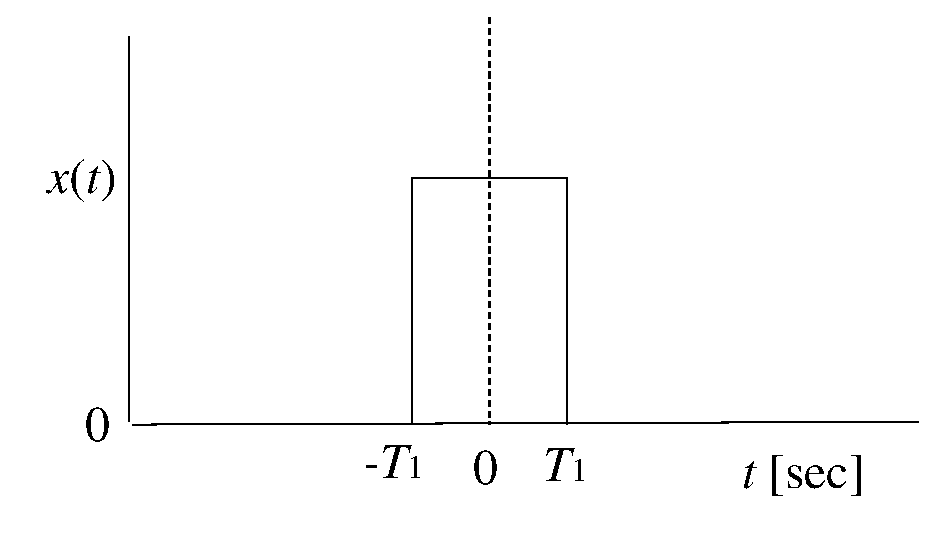
\includegraphics[width=.98\textwidth]{fig/zu-4-13-a.eps}

(a)
\end{center}
\end{minipage}
\begin{minipage}{.35\textwidth}
\begin{center}
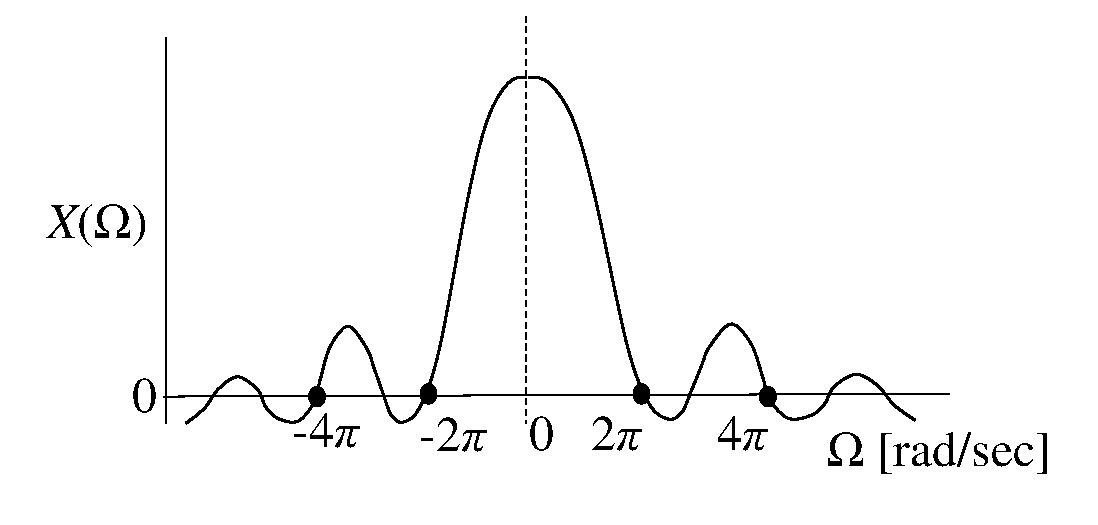
\includegraphics[width=.98\textwidth]{fig/zu-4-13-b.eps}

(b)
\end{center}
\end{minipage}
\end{center}\vskip.5\baselineskip
\caption{非周期信号の例$T_1=0.5$sec}
\label{fig:hishuki-1}
\end{figure}



ここで,式(\ref{eqn:fourier-3_6})はフーリエ変換と呼び,時間領域$x(t)$から周波数領域$X(\Omega)$への変換式である.一方,式(\ref{eqn:inv_fourier-3_1})を逆フーリエ変換と呼び,周波数領域$X(\Omega)$から時間領域$x(t)$への変換式である.また,ここで示したフーリエ変換(式(\ref{eqn:fourier-3_6}))ならびに逆フーリエ変換(式(\ref{eqn:inv_fourier-3_1}))の両式の総称をフーリエ変換と呼ぶこともある.

\subsection*{例題\ref{chapter:6}.3}

図\ref{fig:kukeiha5_6}に示す矩形波について,フーリエ変換せよ.
\begin{equation}
x(t)= \left \{
\begin{array}{ll}
1 & (-T_1 \leq t < T_1) \\
0 & (それ以外)
\end{array}
\right .
\end{equation}


\begin{figure}[H]
\begin{center}
\includegraphics[width=.35\textwidth]{fig/kukeiha.eps}
\caption{矩形波}
\label{fig:kukeiha5_6}
\end{center}
\end{figure}



【解答】式(\ref{eqn:fourier-3_6})より,

\begin{eqnarray}
X(\Omega)&=&\int^{\infty}_{-\infty}x(t)e^{-j\Omega t}d t %\nonumber \\
=\int^{T_1}_{-T_1}e^{-j\Omega t}d t \nonumber %\\
=-\frac{1}{j\Omega} \left ( e^{-j\Omega T_1} - e^{j\Omega T_1} \right ) \nonumber \\
&=&2T_1 \frac{e^{j\Omega T_1} - e^{-j\Omega T_1}}{2j\Omega T_1} %\nonumber \\
=T_1 \mathrm{sinc}(\Omega T_1) 
\end{eqnarray}\vskip.3\baselineskip

\noindent となる\footnotemark .
\footnotetext{sinc関数は信号処理などで多く用いられる関数であり,$\displaystyle \mathrm{sinc}(x)=\frac{\sin x}{x}$と書かれる.なお,$x=0$となる場合には,
\begin{equation}
\displaystyle \lim_{x \to 0}\mathrm{sinc}(x)=\lim_{x \to 0}\frac{\sin x}{x} %\nonumber \\
=\lim_{x \to 0}\frac{\cos x}{1}= 1 \nonumber
\end{equation}
となる.}

\section{\index{さんぷりんぐていり@サンプリング定理}サンプリング定理}

ディジタル信号処理においては,アナログ信号をサンプリングし,ディジタル信号を生成する.その際に,アナログ信号の持つ情報を失わないようにサンプリングを行う必要がある.ここでは,サンプリングに関する問題を扱う.

細かいサンプリング(高いサンプリング周波数)は,データ量を増大させ,その後の処理を複雑にする.一方,粗いサンプリング(低いサンプリング周波数)はデータ量の増大を抑えることはできるが,アナログ信号の持つ情報を失いやすい.したがって,適切なサンプリング周波数の選択が重要となる.

\subsection{帯域制限信号}

まず,図\ref{fig:zu-4-19}(a)に示す振幅スペクトル$A(\Omega)=|X(\Omega)|$を持つアナログ信号$x(t)$を考える.ここで,この信号が
\begin{equation}
|X(\Omega)| = 0, \hspace{1cm} \Omega > \Omega_m
\end{equation}

\begin{figure}[b]
\begin{center}
\begin{minipage}{.35\textwidth}
\begin{center}
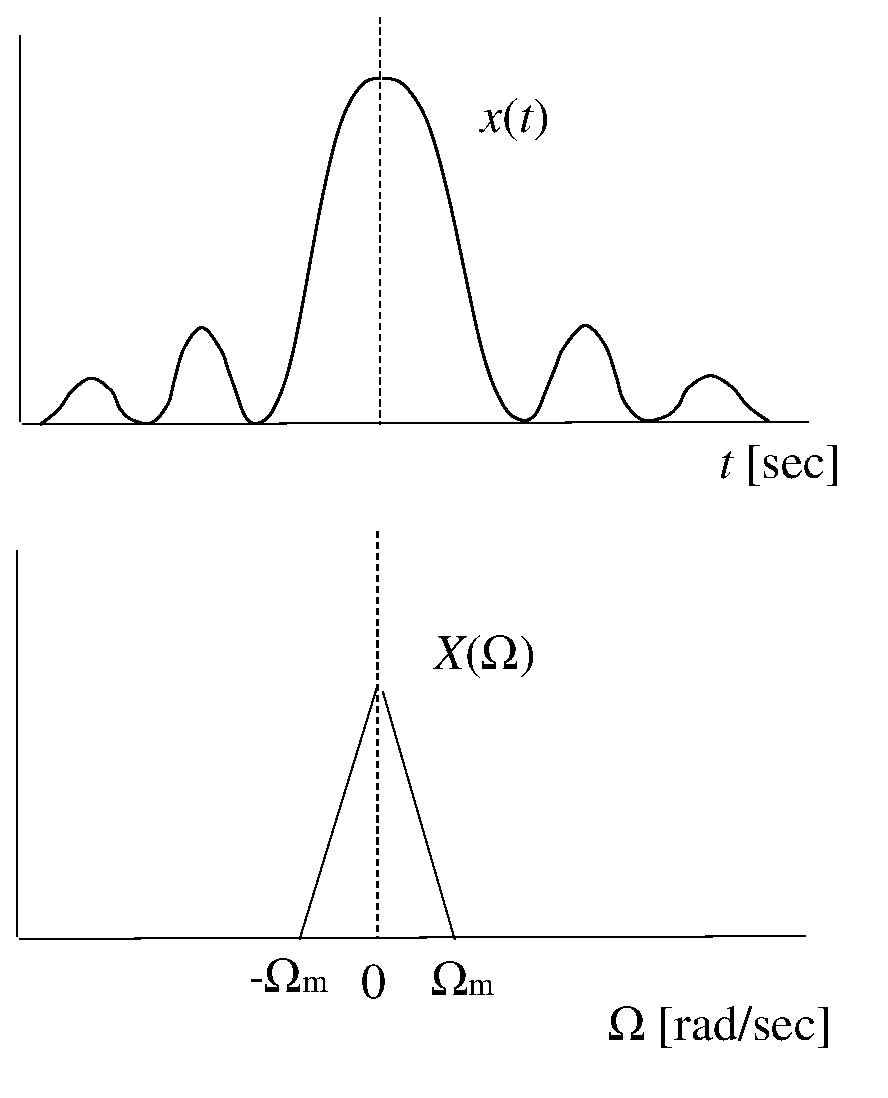
\includegraphics[width=.98\textwidth]{fig/zu-4-19-a.eps}

(a)
\end{center}
\end{minipage}
\begin{minipage}{.35\textwidth}
\begin{center}
\includegraphics[width=.98\textwidth]{fig/zu-4-19-b.eps}

(b)
\end{center}
\end{minipage}\\[.5\baselineskip]
\begin{minipage}{.35\textwidth}
\begin{center}
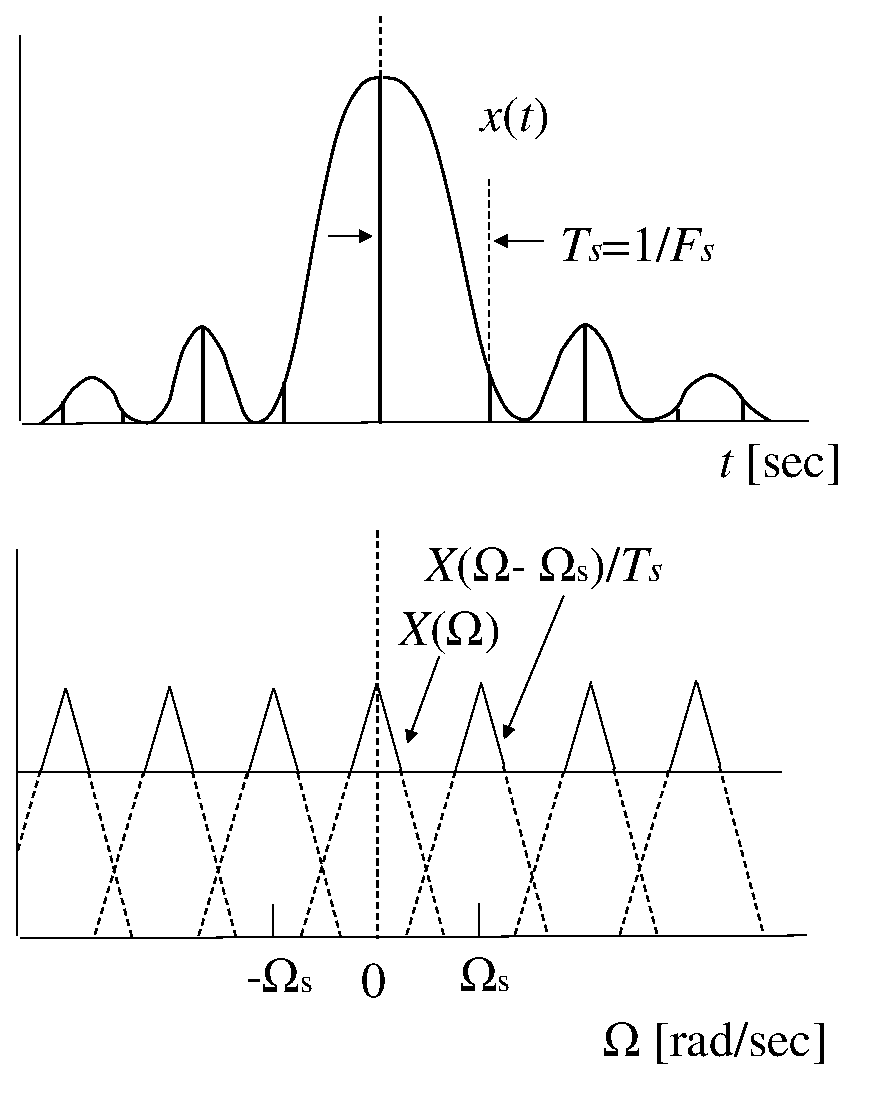
\includegraphics[width=.98\textwidth]{fig/zu-4-19-c.eps}

(c)
\end{center}
\end{minipage}
\end{center}\vskip.5\baselineskip
\caption{矩形波}
\label{fig:zu-4-19}
\end{figure}

\noindent を満たすと仮定する.
%
このとき,信号$x(t)$は,角周波数$\Omega_m=2\pi F_m$(あるいは周波数$F_m$)で帯域制限されているとする.このように,周波数スペクトルの存在する範囲が有限である信号を帯域制限信号という.


\subsection{エリアジング}

次に,信号$x(t)$をサンプリング周波数$F_s=1/T_s$[Hz]でサンプリングするものとして考える.このとき,アナログ信号$x(t)$の周波数スペクトル$X(\Omega)$と離散時間信号$x(nT_s)$の周波数スペクトル$X(e^{j\Omega T_s})$は,次式のような関係で結ばれる.
\begin{equation}
X(e^{j\Omega T_s})=\frac{1}{T_s} \sum_{\tau = -\infty}^{\infty}X(\Omega -r \Omega_s), \hspace{5mm} \Omega_s=2\pi F_s
\end{equation}

図\ref{fig:zu-4-19}をみながらこの式の意味を考えると,以下の事項がわかる.
\begin{itemize}
\item サンプリングすると,アナログ信号のスペクトルが周期的に並ぶ.
\item スペクトルの周期は$\Omega_s = 2\pi F_s$であり,サンプリング周波数$F_s$が高いほど周期は長い.
\item サンプリング周波数が低いほど,スペクトルが重なる場合がある.
\end{itemize}

このようなスペクトルの重なりを,\index{おりかえしひずみ@折り返しひずみ}折り返しひずみあるいは\index{えりあじんぐ@エリアジング}エリアジングという.スペクトルの重なりが生じなければ,離散時間信号はアナログ信号のスペクトルをひずみなく持つことができる.すなわち,この場合,離散時間信号はアナログ信号の情報を失っていないということができる.

\subsection{ナイキスト間隔}

スペクトルの重なりは,信号の帯域$\Omega_m = 2\pi F_m$とサンプリング周波数$F_s=1/T_s$[Hz]との関係から決まる.明らかに,
\begin{equation}
F_s > 2F_m
\end{equation}
であれば,スペクトルの重なりは生じない.

スペクトルの重なる限界であるサンプリング周波数$F_s=2F_m$を\index{ないきすとしゅうはすう@ナイキスト周波数}ナイキスト周波数 (Nquist freauency),その逆数$T_s=1/F_s$をナイキスト間隔という.

\subsection{サンプリング定理}

信号の帯域周波数$F_m$[Hz]で帯域制限された信号$x(t)$は,サンプリング周波数$F_s>2F_m$によるサンプル値で一意に決定される.
%
このことを\index{さんぷりんぐていり@サンプリング定理}サンプリング定理と呼ぶ.スペクトルが重ならないようにサンプリングを行えば,そのサンプル値を用いて元のアナログ信号を復元できることを意味する.この定理により,音声や画像などのメディアをディジタル信号として処理することが可能となる.
\subsection{アナログ--ディジタル変換}

ここまでの議論から,アナログ信号をディジタル信号に変換するためには,図\ref{fig:zu-4-20}に示すような手順が必要であることがわかる.すなわち,
\begin{enumerate}
\item 帯域制限信号を作るために,アナログフィルタより高い周波数スペクトルを除去する.
\item サンプリング定理を満たすサンプリング周波数を選び,サンプリングをする.
\item 各サンプル値を量子化して,ディジタル信号を生成する.
\end{enumerate}

もし帯域制限を行わなければ,サンプリング定理を満たすことができないので,エリアジングが生じる.このため,帯域制限用のアナログフィルタをアンチエリアジングフィルタ (anti-aliasing filter) ということもある.

また,サンプリングおよび量子化の操作をアナログ--ディジタル変換(\index{ADへんかん@A-D変換}A-D変換)といい,そのための装置をアナログ--ディジタル (A-D) 変換器という.逆に,ディジタル信号を再びアナログ信号に変換する操作をディジタル--アナログ変換(\index{D-Aへんかん@D-A変換}D-A変換)といい,そのための装置をディジタル--アナログ (D-A) 変換器という.

\begin{figure}[H]
\begin{center}
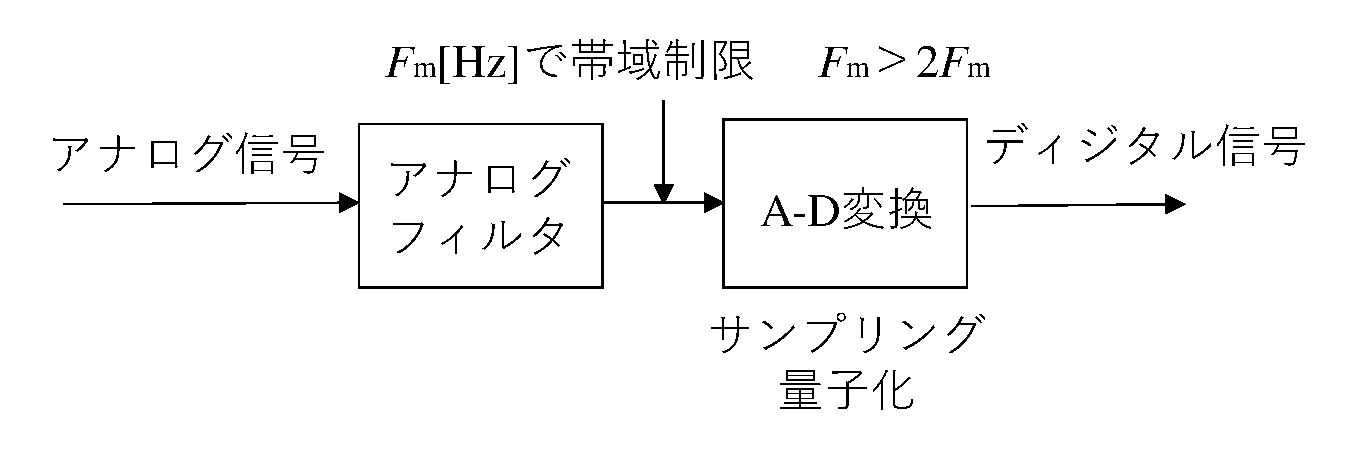
\includegraphics[width=.7\textwidth]{fig/ad-henkan.eps}
\caption{アナログ--ディジタル変換}
\label{fig:zu-4-20}
\end{center}
\end{figure}

\vspace{-\baselineskip}

\section*{演習問題}

\subsection*{問題\ref{chapter:6}.1}

次の離散時間信号におけるフーリエ変換を求めよ.

(1) $x(n)=\delta (nT)$

(2) $x(n)=u (nT)-u(nT-NT)$

\newpage

\subsection*{問題\ref{chapter:6}.2}

図\ref{fig:zu-6e-1}に示す離散時間信号のフーリエ変換を求めよ.

\begin{figure}[H]
\begin{center}
\begin{minipage}{.35\textwidth}
\begin{center}
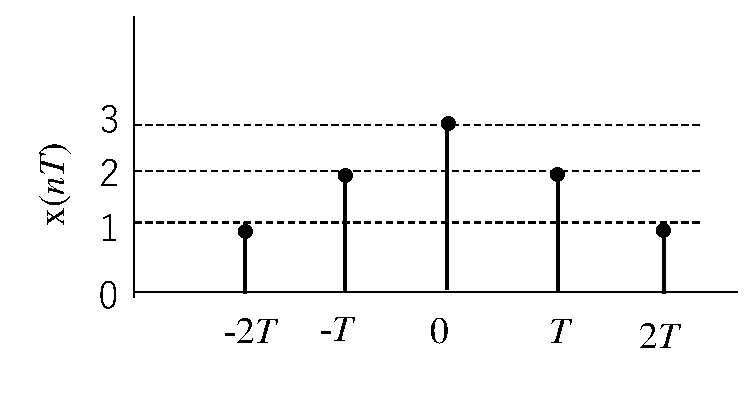
\includegraphics[width=.98\textwidth]{fig/zu-6e-1a.eps}

(a)
\end{center}
\end{minipage}
\begin{minipage}{.35\textwidth}
\begin{center}
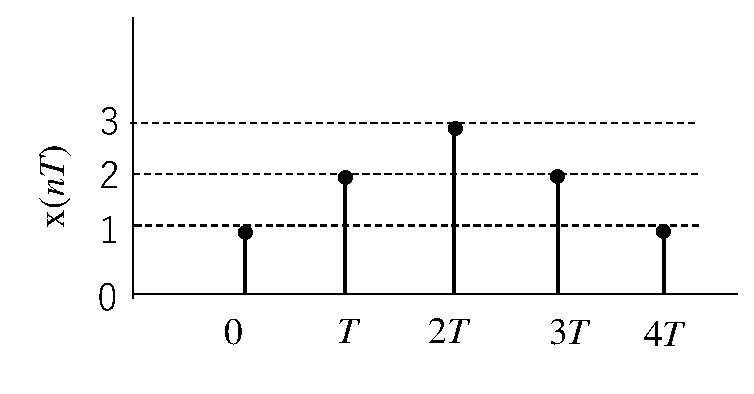
\includegraphics[width=.98\textwidth]{fig/zu-6e-1b.eps}

(b)
\end{center}
\end{minipage}\\[.5\baselineskip]
\begin{minipage}{.35\textwidth}
\begin{center}
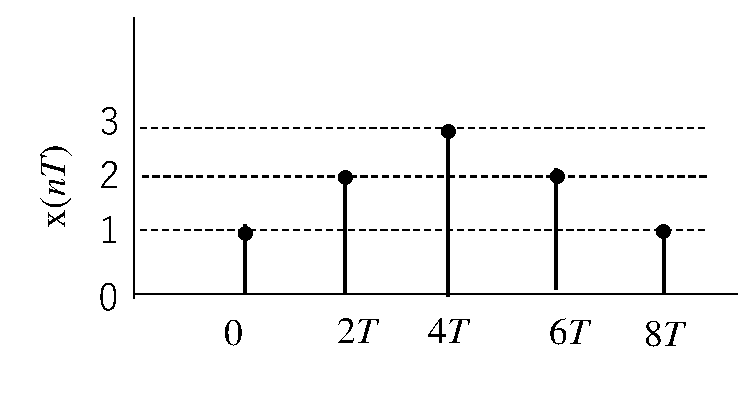
\includegraphics[width=.98\textwidth]{fig/zu-6e-1c.eps}

(c)
\end{center}
\end{minipage}
\end{center}\vskip.5\baselineskip
\caption{問題\ref{chapter:6}.2における離散時間信号}
\label{fig:zu-6e-1}
\end{figure}



\subsection*{問題\ref{chapter:6}.3}

連続時間信号$x(t)=\cos (2\pi f_1 t)+\cos (2\pi f_2 t)$をそのスペクトル情報を乱さないようにサンプリングしたい.その場合,サンプリング周期をどのように設定すればよいか.ただし,$f_1=$1kHz,$f_1=1.5$kHzとする.





